Für arithmetische Ausdrücke mit den Grundoperationen
{\tt +} und {\tt -} stehen die folgenden zwei Grammatiken
zur Auswahl. Einerseits eine leicht abgewandelte Variante
der in der Vorlesung besprochenen Grammatik:
\begin{align*}
\text{Ausdruck}&\rightarrow \text{Zahl}\thickspace\text{'{\tt +}'}\thickspace\text{Ausdruck} \\
               &\rightarrow \text{Zahl}\thickspace\text{'{\tt -}'}\thickspace\text{Ausdruck} \\
               &\rightarrow \text{Zahl}
\end{align*}
Andererseits die folgende Grammatik:
\begin{align*}
\text{Ausdruck}&\rightarrow \text{Term}\thickspace\text{Termsequenz}\\
\text{Termsequenz}&\rightarrow \text{'{\tt +}'}\thickspace \text{Term}\thickspace \text{Termsequenz}\\
                  &\rightarrow \text{'{\tt -}'}\thickspace \text{Term}\thickspace \text{Termsequenz}\\
                  &\rightarrow \varepsilon\\
 \text{Term}&\rightarrow \text{Zahl}
\end{align*}
Die beiden Grammatiken verwenden natürlich die gleichen Regeln
für das nichtterminale Symbol ``Zahl''.
\begin{teilaufgaben}
\item Erstellen Sie für jede Grammatik den parse tree für den Ausdruck
\[
47-1291+1848
\]
\item Formulieren Sie Regeln, wie der arithmetische Ausdruck auf der
Basis des Parse Tree auszuwerten ist.
\item Welche Grammatik ist vorzuziehen?
\end{teilaufgaben}

\thema{Grammatik}
\thema{Parse Tree}

\begin{loesung}
\begin{teilaufgaben}
\item Die erste Grammatik erzeugt
\begin{center}
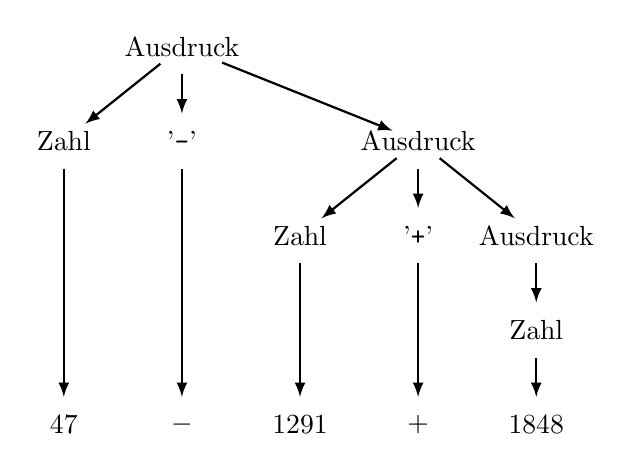
\begin{tikzpicture}[>=latex,thick]
\def\l{1.5}
\def\h{1.2}
\def\pfeil#1#2{
\draw[->,shorten <= 0.35cm,shorten >= 0.35cm] #1 -- #2;
}
\coordinate (p47) at (0,0);
\coordinate (minus) at (\l,0);
\coordinate (p1291) at ({2*\l},0);
\coordinate (plus) at ({3*\l},0);
\coordinate (p1848) at ({4*\l},0);
\coordinate (zahl3) at ({4*\l},\h);
\coordinate (zahl2) at ({2*\l},{2*\h});
\coordinate (pplus) at ({3*\l},{2*\h});
\coordinate (ausdruck3) at ({4*\l},{2*\h});
\coordinate (zahl1) at (0,{3*\h});
\coordinate (mminus) at (\l,{3*\h});
\coordinate (ausdruck2) at ({3*\l},{3*\h});
\coordinate (ausdruck1) at (\l,{4*\h});
\pfeil{(ausdruck1)}{(zahl1)}
\pfeil{(zahl1)}{(p47)}
\pfeil{(ausdruck1)}{(mminus)}
\pfeil{(mminus)}{(minus)}
%\pfeil{(ausdruck1)}{(ausdruck2)}
\draw[->,shorten <= 0.55cm,shorten >= 0.35cm] (ausdruck1) -- (ausdruck2);
\pfeil{(ausdruck2)}{(zahl2)}
\pfeil{(zahl2)}{(p1291)}
\pfeil{(ausdruck2)}{(pplus)}
\pfeil{(pplus)}{(plus)}
\pfeil{(ausdruck2)}{(ausdruck3)}
\pfeil{(ausdruck3)}{(zahl3)}
\pfeil{(zahl3)}{(p1848)}
\node at (ausdruck1) {Ausdruck};
\node at (ausdruck2) {Ausdruck};
\node at (ausdruck3) {Ausdruck};
\node at (zahl1) {Zahl};
\node at (zahl2) {Zahl};
\node at (zahl3) {Zahl};
\node at (p47) {47};
\node at (p1291) {1291};
\node at (p1848) {1848};
\node at (minus) {$-$};
\node at (mminus) {'\texttt{-}'};
\node at (plus) {$+$};
\node at (pplus) {'\texttt{+}'};
\end{tikzpicture}
\end{center}
Bei Verwendung der zweiten Grammatik bekommt man jedoch
\begin{center}
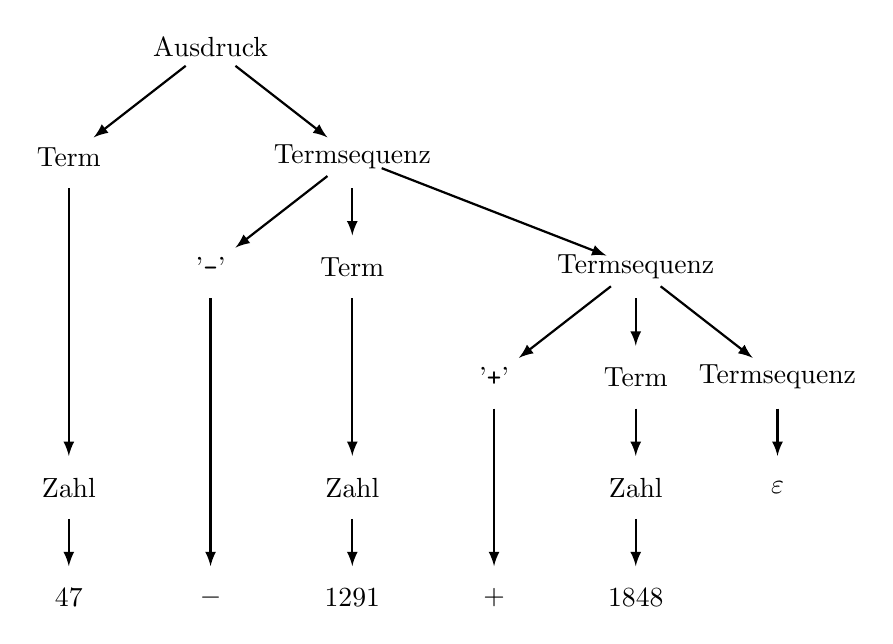
\begin{tikzpicture}[>=latex,thick]
\def\l{1.8}
\def\h{1.4}
\def\pfeil#1#2{
\draw[->,shorten <= 0.4cm,shorten >= 0.4cm] #1 -- #2;
}
\coordinate (p47) at (0,0);
\coordinate (minus) at (\l,0);
\coordinate (p1291) at ({2*\l},0);
\coordinate (plus) at ({3*\l},0);
\coordinate (p1848) at ({4*\l},0);
\node at (p47) {$47$};
\node at (minus) {$-$};
\node at (p1291) {$1291$};
\node at (plus) {$+$};
\node at (p1848) {$1848$};
\coordinate (zahl1) at (0,\h);
\coordinate (zahl2) at ({2*\l},\h);
\coordinate (zahl3) at ({4*\l},\h);
\pfeil{(zahl1)}{(p47)}
\pfeil{(zahl2)}{(p1291)}
\pfeil{(zahl3)}{(p1848)}
\coordinate (pplus) at ({3*\l},{2*\h});
\coordinate (term3) at ({4*\l},{2*\h});
\coordinate (termsequenz3) at ({5*\l},{2*\h});
\coordinate (leer) at ({5*\l},{\h});
\pfeil{(termsequenz3)}{(leer)}
\pfeil{(term3)}{(zahl3)}

\coordinate (mminus) at ({1*\l},{3*\h});
\coordinate (term2) at ({2*\l},{3*\h});
\coordinate (termsequenz2) at ({4*\l},{3*\h});
\pfeil{(term2)}{(zahl2)}
\pfeil{(termsequenz2)}{(pplus)}
\pfeil{(termsequenz2)}{(term3)}
\pfeil{(termsequenz2)}{(termsequenz3)}

\coordinate (term1) at (0,{4*\h});
\coordinate (termsequenz1) at ({2*\l},{4*\h});
\pfeil{(termsequenz1)}{(mminus)}
\pfeil{(termsequenz1)}{(term2)}
\pfeil{(termsequenz1)}{(termsequenz2)}
\pfeil{(term1)}{(zahl1)}

\coordinate (ausdruck) at ({\l},{5*\h});
\pfeil{(ausdruck)}{(term1)}
\pfeil{(ausdruck)}{(termsequenz1)}

\pfeil{(mminus)}{(minus)}
\pfeil{(pplus)}{(plus)}

\node at (ausdruck) {Ausdruck};
\node at (term1) {Term};
\node at (term2) {Term};
\node at (term3) {Term};
\node at (termsequenz1) {Termsequenz};
\node at (termsequenz2) {Termsequenz};
\node at (termsequenz3) {Termsequenz};
\node at (zahl1) {Zahl};
\node at (zahl2) {Zahl};
\node at (zahl3) {Zahl};
\node at (mminus) {'\texttt{-}'};
\node at (pplus) {'\texttt{+}'};
\node at (leer) {$\varepsilon$};
\end{tikzpicture}
\end{center}

\item
Um mit einem Parse Tree einen Ausdruck auszuwerten, muss man für
jede Regel festlegen, wie sie in die Wertberechnung übersetzt werden
muss.

Um für die erste Grammatik festzulegen, wie ein Ausdruck auszuwerten
ist, muss man zuerst den Ausdruck auf der rechten Seite der 
Regel auswerten, und dann die arithmetische Operation mit der Zahl
entsprechend dem Operationszeichen durchführen.

Die Auswertung einer Regel nach der zweiten Grammatik erfolgt anders:
zum Wert der Termsequenz
wird der Wert des Terms hinzuaddiert, mit dem Vorzeichen, das in der
Regel gewählt worden ist.
\item
Für die erste Grammatik wird zuerst die Summe $1291+1848= 3139$
gebildet, die anschliessend von $47$ subtrahiert, was
$
47-(1291+1848)
=
-3092
$
ergibt.
Der erste Parse Tree ergibt also das falsche Resultat.

Das richtige Resultat erhält man jedoch mit dem Parse
Tree nach der zweiten Grammatik.
Von unten nach oben ausgewertet bedeutet das wieder, dass zuerst 
die Termsequenz in der dritten Zeile zu 1848 evaluiert wird.
Die Termsequenz in der zweiten Zeile kann dann als $-1291 + 1848$
ausgerechnet werden. Der Ausdruck ist dann $47$ plus das bisherige
Resultat, also 
$604$, das richtige Resultate.
Daher ist die zweite Grammatik vorzuziehen.
\qedhere
\end{teilaufgaben}
\end{loesung}
